\documentclass[aps,prc,reprint,superscriptaddress,floatfix]{revtex4-2}

\usepackage{graphicx}
\usepackage{amssymb}
\usepackage{amsmath}
\usepackage[version=4]{mhchem}
\usepackage{siunitx}
\usepackage[colorlinks=true,linkcolor=blue,citecolor=blue,urlcolor=blue]{hyperref}

\newcommand{\hide}[1]{}
\newcommand{\myerr}[4]{\SI[parse-numbers=false]{#1^{+#2}_{-#3}}{#4}}

\begin{document}

%\title{\texorpdfstring{Isomeric States in $^{269}$Hs and the Shell Structure near $N=162$ Probed via $^{273}$Ds Decay}{Isomeric States in 269Hs and the Shell Structure near N=162 Probed via 273Ds Decay}}
\title{\texorpdfstring{The Shell Structure near $N=162$ Probed via $^{273}$Ds Decay}{The Shell Structure near N=162 Probed via 273Ds Decay}}

\author{Z. R. Sun}
\affiliation{State Key Laboratory of Heavy Ion Science and Technology, Institute of Modern Physics, Chinese Academy of Sciences, Lanzhou 730000, China}
\affiliation{School of Nuclear Science and Technology, University of Chinese Academy of Sciences, Beijing 100049, China}

\author{M. H. Huang \hide{(黄明辉)}}
\email[Corresponding author: ]{hmh@impcas.ac.cn}
\affiliation{State Key Laboratory of Heavy Ion Science and Technology, Institute of Modern Physics, Chinese Academy of Sciences, Lanzhou 730000, China}
\affiliation{School of Nuclear Science and Technology, University of Chinese Academy of Sciences, Beijing 100049, China}

\author{Z. G. Gan \hide{(甘再国)}}
\email[Corresponding author: ]{zggan@impcas.ac.cn}
\affiliation{State Key Laboratory of Heavy Ion Science and Technology, Institute of Modern Physics, Chinese Academy of Sciences, Lanzhou 730000, China}
\affiliation{School of Nuclear Science and Technology, University of Chinese Academy of Sciences, Beijing 100049, China}
\affiliation{Advanced Energy Science and Technology Guangdong Laboratory, Huizhou 516000, China}

\author{H. B. Yang \hide{(杨华彬)}}
\affiliation{State Key Laboratory of Heavy Ion Science and Technology, Institute of Modern Physics, Chinese Academy of Sciences, Lanzhou 730000, China}
\affiliation{School of Nuclear Science and Technology, University of Chinese Academy of Sciences, Beijing 100049, China}

\author{J. G. Wang \hide{(王建国)}}
\affiliation{State Key Laboratory of Heavy Ion Science and Technology, Institute of Modern Physics, Chinese Academy of Sciences, Lanzhou 730000, China}

\author{Z. Y. Zhang \hide{(张志远)}}
\affiliation{State Key Laboratory of Heavy Ion Science and Technology, Institute of Modern Physics, Chinese Academy of Sciences, Lanzhou 730000, China}
\affiliation{School of Nuclear Science and Technology, University of Chinese Academy of Sciences, Beijing 100049, China}

\author{M. M. Zhang \hide{(张明明)}}
\affiliation{State Key Laboratory of Heavy Ion Science and Technology, Institute of Modern Physics, Chinese Academy of Sciences, Lanzhou 730000, China}
\affiliation{Joint Institute for Nuclear Research, RU-141980 Dubna, Russian Federation}

\author{L. Ma \hide{(马龙)}}
\affiliation{State Key Laboratory of Heavy Ion Science and Technology, Institute of Modern Physics, Chinese Academy of Sciences, Lanzhou 730000, China}
\affiliation{Advanced Energy Science and Technology Guangdong Laboratory, Huizhou 516000, China}

\author{C. L. Yang \hide{(杨春莉)}}
\affiliation{State Key Laboratory of Heavy Ion Science and Technology, Institute of Modern Physics, Chinese Academy of Sciences, Lanzhou 730000, China}

\author{X. L. Wu \hide{(吴晓蕾)}}
\affiliation{State Key Laboratory of Heavy Ion Science and Technology, Institute of Modern Physics, Chinese Academy of Sciences, Lanzhou 730000, China}
\affiliation{Advanced Energy Science and Technology Guangdong Laboratory, Huizhou 516000, China}


\author{Y. L. Tian \hide{(田玉林)}}
\affiliation{State Key Laboratory of Heavy Ion Science and Technology, Institute of Modern Physics, Chinese Academy of Sciences, Lanzhou 730000, China}
\affiliation{Advanced Energy Science and Technology Guangdong Laboratory, Huizhou 516000, China}

\author{Y. S. Wang \hide{(王永生)}}
\affiliation{State Key Laboratory of Heavy Ion Science and Technology, Institute of Modern Physics, Chinese Academy of Sciences, Lanzhou 730000, China}
\affiliation{Advanced Energy Science and Technology Guangdong Laboratory, Huizhou 516000, China}

\author{J. Y. Wang \hide{(王均英)}}
\affiliation{State Key Laboratory of Heavy Ion Science and Technology, Institute of Modern Physics, Chinese Academy of Sciences, Lanzhou 730000, China}
\affiliation{Advanced Energy Science and Technology Guangdong Laboratory, Huizhou 516000, China}

\author{Y. H. Qiang \hide{(强赟华)}}
\affiliation{State Key Laboratory of Heavy Ion Science and Technology, Institute of Modern Physics, Chinese Academy of Sciences, Lanzhou 730000, China}

\author{L. C. Sun \hide{(孙路冲)}}
\affiliation{State Key Laboratory of Heavy Ion Science and Technology, Institute of Modern Physics, Chinese Academy of Sciences, Lanzhou 730000, China}
\affiliation{Shandong Provincial Key Laboratory of Nuclear Science, Nuclear Energy Technology and Comprehensive Utilization, Weihai Frontier Innovation Institute of Nuclear Technology, School of Innovation Science, Energy and Power Engineering, Shandong University, Shandong 250061, People's Republic of China}

\author{X. Zhang \hide{(张旭)}}
\affiliation{State Key Laboratory of Heavy Ion Science and Technology, Institute of Modern Physics, Chinese Academy of Sciences, Lanzhou 730000, China}
\affiliation{School of Nuclear Science and Technology, University of Chinese Academy of Sciences, Beijing 100049, China}

\author{X. Y. Huang \hide{(黄鑫源)}}
\affiliation{State Key Laboratory of Heavy Ion Science and Technology, Institute of Modern Physics, Chinese Academy of Sciences, Lanzhou 730000, China}
\affiliation{School of Nuclear Science and Technology, University of Chinese Academy of Sciences, Beijing 100049, China}

\author{Z. C. Li \hide{(李宗池)}}
\affiliation{State Key Laboratory of Heavy Ion Science and Technology, Institute of Modern Physics, Chinese Academy of Sciences, Lanzhou 730000, China}
\affiliation{School of Nuclear Science and Technology, University of Chinese Academy of Sciences, Beijing 100049, China}

\author{L. Zhu \hide{(祝霖)}}
\affiliation{State Key Laboratory of Heavy Ion Science and Technology, Institute of Modern Physics, Chinese Academy of Sciences, Lanzhou 730000, China}
\affiliation{School of Nuclear Science and Technology, University of Chinese Academy of Sciences, Beijing 100049, China}

\author{H. Zhou \hide{(周浩)}}
\affiliation{State Key Laboratory of Heavy Ion Science and Technology, Institute of Modern Physics, Chinese Academy of Sciences, Lanzhou 730000, China}
\affiliation{School of Nuclear Science and Technology, University of Chinese Academy of Sciences, Beijing 100049, China}

\author{G. Xie \hide{(谢港)}}
\affiliation{State Key Laboratory of Heavy Ion Science and Technology, Institute of Modern Physics, Chinese Academy of Sciences, Lanzhou 730000, China}
\affiliation{School of Nuclear Science and Technology, University of Chinese Academy of Sciences, Beijing 100049, China}

\author{J. H. Zheng \hide{(郑佳卉)}}
\affiliation{State Key Laboratory of Heavy Ion Science and Technology, Institute of Modern Physics, Chinese Academy of Sciences, Lanzhou 730000, China}
\affiliation{School of Nuclear Science and Technology, University of Chinese Academy of Sciences, Beijing 100049, China}

\author{Z. L. Cheng \hide{(程志凌)}}
\affiliation{State Key Laboratory of Heavy Ion Science and Technology, Institute of Modern Physics, Chinese Academy of Sciences, Lanzhou 730000, China}
\affiliation{School of Nuclear Science and Technology, University of Chinese Academy of Sciences, Beijing 100049, China}

\author{Z. H. Li \hide{(李泽浩)}}
\affiliation{State Key Laboratory of Heavy Ion Science and Technology, Institute of Modern Physics, Chinese Academy of Sciences, Lanzhou 730000, China}

\author{W. X. Huang \hide{(黄文学)}}
\affiliation{State Key Laboratory of Heavy Ion Science and Technology, Institute of Modern Physics, Chinese Academy of Sciences, Lanzhou 730000, China}
\affiliation{School of Nuclear Science and Technology, University of Chinese Academy of Sciences, Beijing 100049, China}
\affiliation{Advanced Energy Science and Technology Guangdong Laboratory, Huizhou 516000, China}

\author{Z. W. Lu \hide{(卢子伟)}}
\affiliation{State Key Laboratory of Heavy Ion Science and Technology, Institute of Modern Physics, Chinese Academy of Sciences, Lanzhou 730000, China}

\author{Y. He \hide{(何源)}}
\affiliation{State Key Laboratory of Heavy Ion Science and Technology, Institute of Modern Physics, Chinese Academy of Sciences, Lanzhou 730000, China}
\affiliation{School of Nuclear Science and Technology, University of Chinese Academy of Sciences, Beijing 100049, China}

\author{L. T. Sun \hide{(孙良亭)}}
\affiliation{State Key Laboratory of Heavy Ion Science and Technology, Institute of Modern Physics, Chinese Academy of Sciences, Lanzhou 730000, China}
\affiliation{School of Nuclear Science and Technology, University of Chinese Academy of Sciences, Beijing 100049, China}

\author{Z. Z. Ren \hide{(任中洲)}}
\affiliation{School of Physics Science and Engineering, Tongji University, Shanghai 200092, China}

\author{S. G. Zhou \hide{(周善贵)}}
\affiliation{School of Nuclear Science and Technology, University of Chinese Academy of Sciences, Beijing 100049, China}
\affiliation{CAS Key Laboratory of Theoretical Physics, Institute of Theoretical Physics, Chinese Academy of Sciences, Beijing 100190, China}

\author{V. K. Utyonkov}
\affiliation{Joint Institute for Nuclear Research, RU-141980 Dubna, Russian Federation}

\author{A. A. Voinov}
\affiliation{Joint Institute for Nuclear Research, RU-141980 Dubna, Russian Federation}

\author{Yu. S. Tsyganov}
\affiliation{Joint Institute for Nuclear Research, RU-141980 Dubna, Russian Federation}

\author{A. N. Polyakov}
\affiliation{Joint Institute for Nuclear Research, RU-141980 Dubna, Russian Federation}

\author{D. I. Solovyev}
\affiliation{Joint Institute for Nuclear Research, RU-141980 Dubna, Russian Federation}

\author{N. D. Kovrizhnykh}
\affiliation{Joint Institute for Nuclear Research, RU-141980 Dubna, Russian Federation}

\author{M. V. Shumeiko}
\affiliation{Joint Institute for Nuclear Research, RU-141980 Dubna, Russian Federation}


\date{\today}

\begin{abstract}
The $^{238}$U($^{40}$Ar, $4n$--$5n$)$^{274,273}$Ds reaction was investigated with the SHANS-2 separator at IMP CAS over the excitation-energy range of 42--50 MeV. This reaction had previously been studied at DGFRS-2 in a JINR--IMP CAS experiment at an excitation energy of about 49 MeV, where two $^{273}$Ds decay chains with different $\alpha$-decay energies and lifetimes indicated the possible presence of an isomeric state. In the present measurement, no correlated decay chain was assigned at excitation energies of 42 and 45 MeV, leading to upper cross-section limits of 0.34 and 1.1 pb, respectively. At 50 MeV, two complete decay chains assigned to $^{273}$Ds were observed, giving a $5n$-channel cross section of $0.14^{+0.18}_{-0.08}$ pb, consistent with the value of $0.18^{+0.44}_{-0.12}$ pb reported from DGFRS-2. The new chains extend the decay information for $^{273}$Ds and support the presence of two distinct decay branches. The $\alpha$-particle energies and population pattern of the daughter nucleus $^{269}$Hs further suggest an additional low-energy state, although this assignment remains tentative within the present statistics.
\end{abstract}

\maketitle

\section{Introduction}
\label{introduction}

Without shell stabilization, the macroscopic liquid-drop model would make superheavy elements (SHEs, $Z \ge 104$) unstable against fission because of the large Coulomb repulsion. Their observed existence therefore reflects the stabilizing role of quantum shell effects, which provide additional binding in this mass region. Theoretical models predict that such shell effects give rise to islands of enhanced stability in the superheavy region. Enhanced stability is expected near the deformed shell closures at $Z = 108$ and $N = 162$ \cite{dvorakDoublyMagicNucleus2006}, and toward heavier spherical configurations near $N = 184$ and $Z = 114$--126, although the precise location remains model dependent \cite{kruppa2000ShellCorrectionsSuperheavy}. Odd-$A$ nuclei in this region provide particularly sensitive probes of the single-particle levels that shape the deformed $N = 162$ shell gap. The odd-neutron nucleus $^{273}\mathrm{Ds}$ contains one neutron above this gap, whereas its $\alpha$-decay daughter $^{269}\mathrm{Hs}$ corresponds to one neutron hole below it. The $\alpha$-decay sequence linking $^{273}\mathrm{Ds}$ and $^{269}\mathrm{Hs}$ is therefore a useful probe of the single-particle structure around $N = 162$.

The isotope $^{273}\mathrm{Ds}$ was first identified at the GSI velocity filter SHIP as an $\alpha$-decay product in cold-fusion reactions \cite{hofmann2002NewResultsElements}. In the $^{208}\mathrm{Pb}(^{70}\mathrm{Zn}, n)^{277}\mathrm{Cn}$ cold-fusion experiments at GSI \cite{hofmann2002NewResultsElements,hofmann1996NewElement112} and RIKEN \cite{sumita2013NewResultProduction,morita2007ExperimentSynthesisIsotope277}, the decay times of the $^{273}\mathrm{Ds}$ descendants were consistently of the order of $0.1~\si{ms}$. More recently, direct production of $^{273}\mathrm{Ds}$ through the $^{238}\mathrm{U}(^{40}\mathrm{Ar}, 5n)$ reaction was reported by Oganessian \textit{et al.}~\cite{oganessian2024SynthesisDecayProperties}. Two genetically correlated decay chains were identified \cite{geneticcorrelations}. One chain agreed with previous data, whereas the other was assigned to an isomeric state of $^{273}\mathrm{Ds}$. Because both chains were incomplete, the decay properties of the daughter nucleus $^{269}\mathrm{Hs}$ remained only weakly constrained. Subsequent theoretical analyses based on the DDCM+ and UDF approaches led to minor proposed revisions of the assigned decay paths \cite{Wang2024}. In the present work, the same reaction was studied at the SHANS-2 facility \cite{xu2023GasfilledRecoilSeparator}, and two additional complete decay chains assigned to $^{273}\mathrm{Ds}$ were observed. Together with the earlier data, these chains support the existence of two distinct states in $^{273}\mathrm{Ds}$, denoted here as $^{273}\mathrm{Ds}^{a}$ and $^{273}\mathrm{Ds}^{b}$ following Ref.~\cite{oganessian2024SynthesisDecayProperties}.

Using the decay chains observed in the present work and the available literature data, we examine the evidence for isomerism in $^{273}\mathrm{Ds}$ and discuss a possible additional low-energy state in $^{269}\mathrm{Hs}$. The implications for the neutron single-particle structure around the deformed $N = 162$ shell gap are discussed with guidance from macroscopic--microscopic calculations.

\section{Experiment and results}

The experiment was performed at China Accelerator Facility for superheavy Elements (CAFE2)\cite{sheng2021IonopticalDesignMultiparticle} of Institute of Modern Physics, Chinese Academy of Sciences (IMP) , by using the Spectrometer for Heavy Atoms and Nuclear Structure-2 (SHANS-2) gas-filled recoil separator\cite{xu2023GasfilledRecoilSeparator}. The nucleus $^{273}\mathrm{Ds}$ was produced through the $^{238}\mathrm{U}(^{40}\mathrm{Ar}, 5n)$ fusion-evaporation reaction. The $^{40}\mathrm{Ar}^{13+}$ beam with average laboratory energies of 217, 220, and 225 MeV was delivered by a superconducting linear accelerator. The beam intensity on target was typically about $5\ \mathrm{p}\mu\mathrm{A}$, and the total effective irradiation time was about 655 h.%728*0.9

The targets were prepared by magnetron sputtering $^{238}\mathrm{U}$ onto Ti backings with thicknesses of 2.22 and 2.19 $\mu\mathrm{g/cm}^{2}$. The resulting average $^{238}\mathrm{U}$ layer thicknesses were 470 and 604 $\mu\mathrm{g/cm}^{2}$. The arc-shaped target segments were mounted on a wheel with a diameter of 50 cm, which rotated at 1500 rpm during irradiation.%to reduce beam-induced damage.

Evaporation residues were separated in flight from the primary beam and other reaction products by SHANS-2. The separator was filled with helium gas at a pressure of about 1 mbar, and the magnetic rigidity was optimized for the transmission of $^{273}\mathrm{Ds}$ and $^{274}\mathrm{Ds}$. At the focal plane, the evaporation residues first passed through two multi-wire proportional chambers(MWPCs) before being implanted into a double-sided silicon strip detector(DSSD). The MWPCs were mounted about 20 cm upstream of the implantation detector and were operated with iso-butane gas. They were used to distinguish implantation events from decay events through time--position correlations, together with time-of-flight information and the chamber trigger condition.

The DSSD has an active area of $128 \times 48\ \mathrm{mm}^{2}$ and a thickness of 300 \si{\um}. Its front side, which served as the implantation face and is defined as the Y-position, is divided into 48 horizontal strips. 
The rear side, defined as the X-position, is divided into 128 vertical strips. This configuration forms 6144 pixels and provides a position resolution of about 1 mm. 
Six single-sided silicon detectors(SSDs) were arranged upstream of the DSSD in an open box-like geometry to detect $\alpha$ particles and spontaneous-fission fragments escaping from the DSSD. 
Each single-sided detector has a thickness of 500 \si{\um} and an active area of $120 \times 63\ \mathrm{mm}^{2}$. 
Three silicon detectors with a thickness of 300 \si{\um} were installed immediately behind the implantation detector as Veto detectors to exclude light particles punching through the focal-plane detectors. 
The silicon detector array was cooled to approximately $\SI{-30}{\celsius}$ with a circulating liquid-alcohol system to reduce thermal noise and improve energy resolution. 
For full-energy $\alpha$ particles in the 5--9 MeV range, the typical energy resolution of the implantation detector was about 30 keV FWHM. The $\alpha$-particle detection efficiency was about 87(6)\%. 
All detector signals, after preamplification and shaping, were recorded by 14-bit analog-to-digital converters operated at a sampling rate of 100 MHz in triggerless mode. Further details of SHANS-2 and the detection system are given in Refs.~\cite{xu2023GasfilledRecoilSeparator,sheng2021IonopticalDesignMultiparticle}.

The silicon detectors were calibrated with standard $\alpha$ sources \ce{^{239}Pu}, \ce{^{241}Am}, and \ce{^{244}Cm}, and with well-known $\alpha$-decay lines of \ce{^{218}Rn} \cite{SINGH2019405}, \ce{^{214}Po} \cite{ZHU20211a}, \ce{^{216}Po} \cite{WU20071057}, and \ce{^{217}At} \cite{KONDEV2018382}.
Cross sections were deduced with simulations following the method described in Ref.~\cite{zhang2026MonteCarloSimulation}, which gave a transmission efficiency of 20\%. 
% Transmission efficiency were deduced with ${}^{48}\mathrm{Ca}+{}^{208}\mathrm{Pb}$ in Ref.~\cite{ZXTran}, which gave a transmission efficiency of 67(11)\%. 
The experimental conditions and measured cross sections are summarized in Table~\ref{tab:cross_sections}.

\begin{table}[htbp]
\centering
\caption{The $^{238}$U target thicknesses, average laboratory-frame projectile energies $\bar{E}_{\rm lab}$ at the middle of the target layers, corresponding average excitation energies $\bar{E}^{*}$ of the compound nucleus calculated using the mass tables of Refs.~\cite{myers1996NuclearPropertiesAccording,wang2021NUBASE2020EvaluationNuclear}, total beam doses, and measured cross sections $\sigma$ or upper limits for the $4n$- and $5n$-evaporation channels in the $^{40}$Ar + $^{238}$U reaction. Values separated by ``$|$'' denote measurements performed with two different target thicknesses; the corresponding beam doses are listed in the same order.}
\label{tab:cross_sections}
\footnotesize
\begin{ruledtabular}
\begin{tabular}{@{}cccccc@{}}
Target thickness & $\bar{E}_{\rm lab}^{\mathrm{a}}$ & $\bar{E}^{*}$ & Beam dose & $\sigma_{4n}$ & $\sigma_{5n}$ \\
(mg/cm$^{2}$) & (MeV) & (MeV) & ($\times 10^{19}$) & (pb) & (pb) \\
\colrule
\noalign{\vskip 1pt}
$0.47\,|\,0.60$ & 225 & 50 & $2.28\,|\,2.96$ & $<0.15$ & $0.14^{+0.18}_{-0.08}$ \\
0.47            & 220 & 45 & 0.817           & $<1.1$  & $<1.1$ \\
0.60            & 217 & 42 & 2.04            & $<0.34$ & $<0.34$ \\
\end{tabular}
\end{ruledtabular}
\begin{flushleft}
\footnotesize \textsuperscript{a} The beam energy was measured with a systematic uncertainty of 1 MeV.
\end{flushleft}
\end{table}
% \begin{table}[htbp]
% \centering
% \caption{The $^{238}$U target thicknesses, average laboratory-frame projectile energies $\bar{E}_{\rm lab}$ at the middle of the target layers, corresponding average excitation energies $\bar{E}^{*}$ of the compound nucleus calculated using the mass tables of Refs.~\cite{myers1996NuclearPropertiesAccording,wang2021NUBASE2020EvaluationNuclear}, total beam doses, and measured cross sections $\sigma$ or upper limits for the $4n$- and $5n$-evaporation channels in the $^{40}$Ar + $^{238}$U reaction. Values separated by ``$|$'' denote measurements performed with two different target thicknesses; the corresponding beam doses are listed in the same order.}
% \label{tab:cross_sections}
% \footnotesize
% \begin{ruledtabular}
% \begin{tabular}{@{}cccccc@{}}
% Target thickness & $\bar{E}_{\rm lab}^{\mathrm{a}}$ & $\bar{E}^{*}$ & Beam dose & $\sigma_{4n}$ & $\sigma_{5n}$ \\
% (mg/cm$^{2}$) & (MeV) & (MeV) & ($\times 10^{19}$) & (fb) & (fb) \\
% \colrule
% \noalign{\vskip 1pt}
% $0.47\,|\,0.60$ & 225 & 50 & $2.28\,|\,2.96$ & $<43$ & $41^{+55}_{-28}$ \\
% 0.47            & 220 & 45 & 0.817           & $<325$  & $<325$ \\
% 0.60            & 217 & 42 & 2.04            & $<102$  & $<102$ \\
% \end{tabular}
% \end{ruledtabular}
% \begin{flushleft}
% \footnotesize \textsuperscript{a} The beam energy was measured with a systematic uncertainty of 1 MeV.
% \end{flushleft}
% \end{table}

\section{Decay-chain assignments}

For the $^{238}\mathrm{U}(^{40}\mathrm{Ar}, xn)^{278-x}\mathrm{Ds}$ reaction at an excitation energy of approximately 50 MeV, the $5n$ evaporation channel is expected to be dominant \cite{oganessian2024SynthesisDecayProperties}. At this excitation energy, two decay chains assigned to $^{273}\mathrm{Ds}$ were observed, as shown in Fig.~\ref{fig:decay-chain}.

\begin{figure}
\centering

\includegraphics[width=0.4\textwidth]{decayChain.pdf}
\caption{Two decay chains assigned to $^{273}$Ds observed in the $^{238}$U($^{40}$Ar, $5n$)$^{273}$Ds reaction. For each chain, the energy of the evaporation-residue event and the corresponding $X/Y$ detector position are shown at the top, followed by the energies of successive $\alpha$-decay events and the terminal spontaneous-fission event, together with the time intervals between adjacent events. Energies in parentheses denote summed signals. Italic values indicate the corresponding energy uncertainties. Red text and red-framed entries highlight the information validated in the present work and the inferred assignments associated with the proposed isomeric states.}
\label{fig:decay-chain}
\end{figure}

The $\alpha_{1}$ energy and correlation time in Chain 1 are consistent with the values reported in previous cold-fusion $^{208}\mathrm{Pb}(^{70}\mathrm{Zn}, n)^{277}\mathrm{Cn}$ experiments at GSI \cite{hofmann2002NewResultsElements,hofmann1996NewElement112} and RIKEN \cite{sumita2013NewResultProduction,morita2007ExperimentSynthesisIsotope277}, as well as with those reported in the hot-fusion $^{238}\mathrm{U}(^{40}\mathrm{Ar}, 5n)^{273}\mathrm{Ds}$ experiment at JINR \cite{oganessian2024SynthesisDecayProperties}. The subsequent decays of $^{269}\mathrm{Hs}$ and $^{265}\mathrm{Sg}$, together with the terminal spontaneous fission of $^{261}\mathrm{Rf}$, are also consistent with decay data reported in Refs.~\cite{dvorakDoublyMagicNucleus2006,dullmannCm248Ne2008,dvorakObservation3Evaporation2008,graegerExperimentalStudy2382010,vonzweidorfEvidenceFormationSodium2004,habaProductionDecayProperties2011,habaProduction265Sg2012}.

D\"ullmann \textit{et al.}~\cite{dullmannCm248Ne2008} proposed that $^{261}\mathrm{Rf}$ populated by the $\alpha$ decay of $^{265}\mathrm{Sg}$ contains two states, denoted as $^{261}\mathrm{Rf}^{a}$ and $^{261}\mathrm{Rf}^{b}$. The existence and decay properties of these states were later confirmed by Haba \textit{et al.}~\cite{habaProductionDecayProperties2011} in the $^{248}\mathrm{Cm}(^{18}\mathrm{O}, 5n)^{261}\mathrm{Rf}$ reaction. The state $^{261}\mathrm{Rf}^{a}$ decays to $^{257}\mathrm{No}$ through emission of an $8.28\pm0.02~\si{MeV}$ \cite{firestone_2025_ahwst-0j467} $\alpha$ particle, with $T_{1/2} = 68\pm 3~\si{s}$ \cite{habaProduction265Sg2012}. In contrast, $^{261}\mathrm{Rf}^{b}$ has $T_{1/2} = \myerr{2.6}{0.7}{0.5}{s}$ and decays through an $18\pm9\%$ $\alpha$ branch with $E_{\alpha} = 8.51\pm0.06~\si{MeV}$ to $^{257}\mathrm{No}$, together with an $82\pm9\%$ spontaneous-fission branch \cite{habaProductionDecayProperties2011}. On this basis, the terminal spontaneous-fission events observed in the two chains of the present work are assigned to $^{261}\mathrm{Rf}^{b}$.

J. Dvorak \textit{et al.}~\cite{dvorakDoublyMagicNucleus2006} reported that the $\alpha$ decay of $^{269}\mathrm{Hs}$ proceeds through two $\alpha$-particle energies, $E_{\alpha} = 9.13\pm0.05$ and $8.95\pm0.05~\si{MeV}$, which populate two states in the daughter nucleus, $^{265}\mathrm{Sg}^{a}$ and $^{265}\mathrm{Sg}^{b}$. These energies agree with the $E_{\alpha_{2}}$ values observed in Chains 1 and 2. The decay properties of $^{265}\mathrm{Sg}^{a}$ and $^{265}\mathrm{Sg}^{b}$ were established by Haba \textit{et al.}~\cite{habaProduction265Sg2012} using high-statistics data from the $^{248}\mathrm{Cm}(^{22}\mathrm{Ne}, 5n)^{265}\mathrm{Sg}$ reaction. They found that $^{265}\mathrm{Sg}^{a}$, with $T_{1/2} = \myerr{8.5}{2.6}{1.6}{s}$, decays through an $8.84 \pm 0.05~\si{MeV}$ $\alpha$ emission and feeds $^{261}\mathrm{Rf}^{a}$ and $^{261}\mathrm{Rf}^{b}$ with branching ratios of 91\% and 9\%, respectively. By comparison, $^{265}\mathrm{Sg}^{b}$, with $T_{1/2} = \myerr{14.4}{3.7}{2.5}{s}$, decays through an $8.69 \pm 0.05~\si{MeV}$ $\alpha$ emission and feeds $^{261}\mathrm{Rf}^{a}$ and $^{261}\mathrm{Rf}^{b}$ with branching ratios of 20\% and 80\%, respectively. The observed $E_{\alpha_{3}}$ values, together with the terminal spontaneous-fission assignments to $^{261}\mathrm{Rf}^{b}$, therefore support the assignment of both chains to the $^{265}\mathrm{Sg}^{b} \rightarrow {}^{261}\mathrm{Rf}^{b}$ decay sequence. The $E_{\alpha}$ and $\tau$ values for decay chains involving \ce{^{273}Ds} are compared with previous data in Fig.~\ref{fig:EalphaAndDecaytime}.

% \begin{figure}
% \centering
% 
\includegraphics[width=0.48\textwidth]{EalphaAndDecaytime.pdf}
% \caption{Comparison of $E_{\alpha}$ and half-life information for decay chains involving $^{273}$Ds. The red, blue, green, and yellow symbols correspond to IMP, JINR \cite{oganessian2024SynthesisDecayProperties}, RIKEN \cite{sumita2013NewResultProduction,morita2007ExperimentSynthesisIsotope277}, and GSI \cite{hofmann2002NewResultsElements,hofmann1996NewElement112}, respectively. The fitted curves in the decay-time panels are drawn following Ref.~\cite{schmidt2000NewTestRandom}.}
% \label{fig:EalphaAndDecaytime}
% \end{figure}
\begin{figure}
\centering

\includegraphics[width=0.48\textwidth]{EalphaAndDecaytime.pdf}
\caption{Comparison of $E_{\alpha}$ (a)-(d) and half-life (e)-(h) information for decay chains involving $^{273}$Ds. The red, blue, green, and yellow symbols correspond to IMP, JINR \cite{oganessian2024SynthesisDecayProperties}, RIKEN \cite{sumita2013NewResultProduction,morita2007ExperimentSynthesisIsotope277}, and GSI \cite{hofmann2002NewResultsElements,hofmann1996NewElement112}, respectively. 
The fitted curves in the (e)-(h) are drawn following Ref.~\cite{schmidt2000NewTestRandom}.}
\label{fig:EalphaAndDecaytime}
\end{figure}

\subsection{\texorpdfstring{Decay properties of~ $^{273}\mathrm{Ds}$}{Decay properties of 273Ds}}
%\subsection{Decay properties of $^{273}\mathrm{Ds}$ }

As shown in Fig.~\ref{fig:EalphaAndDecaytime}, most decay data for Chains 1 and 2 in the present work are consistent with previous measurements. The reported $^{273}\mathrm{Ds}$ event from Ref.~\cite{oganessian2024SynthesisDecayProperties}, with $E_{\alpha} = 10.929(22)~\si{MeV}$ and $\tau = 41.703~\si{ms}$, and the present event with $E_{\alpha} = 10.858(22)~\si{MeV}$ and $\tau = 8.320~\si{ms}$ differ from the higher-energy, shorter-lived decays observed at GSI and RIKEN. Figure~\ref{fig:EalphaAndDecaytime}(e) reveals a further noticeable deviation in the decay-time distribution of $^{273}\mathrm{Ds}$. The seven higher-energy, short-lived events, give a fitted half-life of $T_{1/2}=0.16^{+0.08}_{-0.05}~\si{ms}$. Based on this activity, only $3.7\times10^{-15}$ events with $\tau \geq 8.320~\si{ms}$ would be expected among the nine available events, instead of the two observed. These two lower-energy events with $\tau$ values of 8.320 ms and 41.703 ms may therefore originate from a different state in $^{273}\mathrm{Ds}$. Within the present statistics, this separation supports a candidate long-lived, lower-energy isomeric state in $^{273}\mathrm{Ds}$.

The nucleus $^{273}\mathrm{Ds}$ can be populated either as an $\alpha$-decay daughter of $^{277}\mathrm{Cn}$ produced in the cold-fusion $^{208}\mathrm{Pb}(^{70}\mathrm{Zn}, n)$ reaction at GSI \cite{hofmann2002NewResultsElements,hofmann1996NewElement112} and RIKEN \cite{sumita2013NewResultProduction,morita2007ExperimentSynthesisIsotope277}, or directly through the hot-fusion $^{238}\mathrm{U}(^{40}\mathrm{Ar}, 5n)$ reaction at JINR \cite{oganessian2024SynthesisDecayProperties} and in the present work. The available data show two groups of $\alpha$-decay energies and lifetimes for $^{273}\mathrm{Ds}$. Following Ref.~\cite{oganessian2024SynthesisDecayProperties}, the lower-energy, longer-lived branch is denoted as $^{273}\mathrm{Ds}^{a}$, whereas the higher-energy branch is denoted as $^{273}\mathrm{Ds}^{b}$. So far, $^{273}\mathrm{Ds}$ populated through the $\alpha$ decay of $^{277}\mathrm{Cn}$ has been observed only in the $^{273}\mathrm{Ds}^{a}$ branch, whereas direct production populates both branches with comparable yields. This population pattern supports the assignment of $^{273}\mathrm{Ds}^{a}$ as a candidate isomeric state.

% \subsection{\texorpdfstring{Decay properties of~ $^{269}\mathrm{Hs}$}{Decay properties of 269Hs}}

% T\"urler \textit{et al.}~\cite{turlerNuclearStructureReaction2012} noted that the $\alpha$-decay energies of $^{269}\mathrm{Hs}$ observed as descendants of $^{277}\mathrm{Cn}$ and $^{273}\mathrm{Ds}$, $9.17$--$9.25$ MeV, are among the highest reported for this nuclide. They suggested two possible explanations: energy summing with conversion electrons in focal-plane implantation events, or the presence of long-lived isomeric states in $^{269}\mathrm{Hs}$, similar to those known in $^{265}\mathrm{Sg}$ and $^{261}\mathrm{Rf}$. In view of the present $^{269}\mathrm{Hs}$ decay information, the $\alpha$-energy distribution is shown in Fig.~\ref{fig:distributionHs}. Following the notation of Oganessian \textit{et al.}~\cite{oganessian2024SynthesisDecayProperties}, the group with $E_{\alpha} = 9.20(4)\ \mathrm{MeV}$ and $T_{1/2} = 13^{+10}_{-4}\ \mathrm{s}$ is denoted as $^{269}\mathrm{Hs}^{a}$, and the group with $E_{\alpha} = 9.08(15)\ \mathrm{MeV}$ and $T_{1/2} = 2.8^{+13.6}_{-1.3}\ \mathrm{s}$ is denoted as $^{269}\mathrm{Hs}^{b}$. The present event with $E_{\alpha} = 8.915(22)\ \mathrm{MeV}$ and $\tau = 9.363\ \mathrm{s}$ is assigned to a third tentative group, $^{269}\mathrm{Hs}^{c}$. Because part of the historical data has limited energy resolution, the distinction between $^{269}\mathrm{Hs}^{a}$ and $^{269}\mathrm{Hs}^{b}$ is not always clear; where appropriate, these two groups are therefore denoted collectively as $^{269}\mathrm{Hs}^{a+b}$.

% \begin{figure}
% \centering
% 
\includegraphics[width=0.4\textwidth]{distributionHs.pdf}
% \caption{Energy distributions of $\alpha$ particles assigned to $^{269}$Hs. The upper panel shows all events, the middle panel shows nuclei produced directly as evaporation residues, and the lower panel shows nuclei populated through the $\alpha$ decay of $^{273}$Ds.
% The hatched bar indicates the event observed in the present work at $E_{\alpha} = 8.915$ MeV,which corresponds to the $\alpha$ decay of $^{269}$Hs originating from $^{273}\mathrm{Ds}^{a}$.
% Data sourced from Refs.~\cite{hofmann2002NewResultsElements,hofmann1996NewElement112,sumita2013NewResultProduction,morita2007ExperimentSynthesisIsotope277,dullmannCm248Ne2008,dvorakDoublyMagicNucleus2006,dvorakObservation3Evaporation2008,vonzweidorfEvidenceFormationSodium2004,turlerNuclearStructureReaction2012}.}

% \label{fig:distributionHs}
% \end{figure}

% As shown in Fig.~\ref{fig:distributionHs}, $^{269}\mathrm{Hs}$ nuclei produced directly as evaporation residues populate all three groups. With 9.0 MeV used as an energy boundary, the population ratio is $n(^{269}\mathrm{Hs}^{a+b}):n(^{269}\mathrm{Hs}^{c}) = 11:5$.
% For $^{269}\mathrm{Hs}$ populated through the $\alpha$ decay of $^{273}\mathrm{Ds}$, the corresponding ratio is $n(^{269}\mathrm{Hs}^{a+b}):n(^{269}\mathrm{Hs}^{c}) = 6:1$. In this latter set, the event assigned to $^{269}\mathrm{Hs}^{c}$ is connected with the candidate isomeric branch $^{273}\mathrm{Ds}^{a}$, whereas the higher-energy events are associated with $^{273}\mathrm{Ds}^{b}$. The corresponding ratio is therefore $n(^{273}\mathrm{Ds}^{b} \rightarrow {}^{269}\mathrm{Hs}^{a+b}):n(^{273}\mathrm{Ds}^{a} \rightarrow {}^{269}\mathrm{Hs}^{c}) = 6:1$. No cross feeding of the types $^{273}\mathrm{Ds}^{b} \rightarrow {}^{269}\mathrm{Hs}^{c}$ or $^{273}\mathrm{Ds}^{a} \rightarrow {}^{269}\mathrm{Hs}^{a+b}$ is observed in the present data. This selectivity suggests that $^{269}\mathrm{Hs}^{c}$ may represent an additional low-lying state, although further experimental and theoretical support is required.

% To examine, in purely statistical terms, whether the high-energy $^{269}$Hs data are better represented by one peak or two, we performed a Gaussian-mixture maximum-likelihood analysis \cite{mclachlan2004MixtureModellingCluster}, using fixed measurement uncertainties for the individual data points. For the high-energy subset ($E_{\alpha} > 9.0$ MeV), the single-peak fit gives $\log L=-141.58$, $\mathrm{AIC}=285.15$, and $\mathrm{BIC}=285.92$, with a centroid at 9.165 MeV. The two-component fit gives $\log L=-93.53$, $\mathrm{AIC}=193.06$, and $\mathrm{BIC}=195.38$, with centroids at $9.108 \pm 0.010$ and $9.199 \pm 0.015$ MeV. The likelihood-ratio improvement, $\mathrm{LR}=96.09$, is therefore very large, and in the present analysis the two-component description is further favored by the parametric-bootstrap test \cite{mclachlan1987BootstrappingLikelihoodRatio}. This mathematical analysis, however, should be regarded only as supportive rather than decisive evidence. It does not by itself distinguish unresolved fine-structure $\alpha$ decay from decays originating from distinct isomeric states; it only indicates that the observed high-energy distribution is better described by a two-peak model than by a single-peak one. The labels $^{269}\mathrm{Hs}^{a}$ and $^{269}\mathrm{Hs}^{b}$ used below therefore denote tentative classes defined from the larger posterior membership probability of each datum. In view of the limited statistics and the heterogeneous energy resolution of the combined data set, this subdivision should still be regarded as provisional.

\subsection{\texorpdfstring{Decay properties of~ $^{269}\mathrm{Hs}$}{Decay properties of 269Hs}}

T\"urler \textit{et al.}~\cite{turlerNuclearStructureReaction2012} noted that the $\alpha$-decay energies of $^{269}\mathrm{Hs}$ observed in decay chains from $^{277}\mathrm{Cn}$ and $^{273}\mathrm{Ds}$, $9.17$--$9.25~\si{MeV}$, are among the highest values reported for this nuclide. They proposed two possible explanations: energy summing with conversion electrons in focal-plane implantation events, or the presence of long-lived isomeric states in $^{269}\mathrm{Hs}$, analogous to those known in $^{265}\mathrm{Sg}$ and $^{261}\mathrm{Rf}$. To place the present $^{269}\mathrm{Hs}$ decay information in this context, the $\alpha$-energy distribution is shown in Fig.~\ref{fig:distributionHs}. Following the notation used by Oganessian \textit{et al.}~\cite{oganessian2024SynthesisDecayProperties}, the group with $E_{\alpha}=9.20(4)~\si{MeV}$ and $T_{1/2}=13^{+10}_{-4}~\si{s}$ is denoted as $^{269}\mathrm{Hs}^{a}$, whereas the group with $E_{\alpha}=9.08(15)~\si{MeV}$ and $T_{1/2}=2.8^{+13.6}_{-1.3}~\si{s}$ is denoted as $^{269}\mathrm{Hs}^{b}$. The present event, with $E_{\alpha}=8.915(22)~\si{MeV}$ and $\tau=9.363~\si{s}$, is assigned to a third tentative group, $^{269}\mathrm{Hs}^{c}$. Because some measurements have limited energy resolution, the separation between $^{269}\mathrm{Hs}^{a}$ and $^{269}\mathrm{Hs}^{b}$ is not always unambiguous. When such a separation is not required, these two groups are therefore denoted collectively as $^{269}\mathrm{Hs}^{a+b}$.

\begin{figure}
\centering

\includegraphics[width=0.4\textwidth]{distributionHs.pdf}
\caption{Energy distributions of $\alpha$ particles assigned to $^{269}\mathrm{Hs}$. The upper panel shows the full set of events, the middle panel shows nuclei produced directly as evaporation residues, and the lower panel shows nuclei populated through the $\alpha$ decay of $^{273}\mathrm{Ds}$.
The hatched bar marks the event observed in the present work at $E_{\alpha}=8.915(22)~\si{MeV}$, which corresponds to the $\alpha$ decay of $^{269}\mathrm{Hs}$ populated from $^{273}\mathrm{Ds}^{a}$.
Data are taken from Refs.~\cite{hofmann2002NewResultsElements,hofmann1996NewElement112,sumita2013NewResultProduction,morita2007ExperimentSynthesisIsotope277,dullmannCm248Ne2008,dvorakDoublyMagicNucleus2006,dvorakObservation3Evaporation2008,vonzweidorfEvidenceFormationSodium2004,turlerNuclearStructureReaction2012}.}

\label{fig:distributionHs}
\end{figure}

% As shown in Fig.~\ref{fig:distributionHs}, $^{269}\mathrm{Hs}$ nuclei produced directly as evaporation residues populate all three groups. Using $E_{\alpha}=9.0\ \mathrm{MeV}$ as a practical boundary, the population ratio is $n(^{269}\mathrm{Hs}^{a+b}):n(^{269}\mathrm{Hs}^{c})=11:5$. For $^{269}\mathrm{Hs}$ nuclei populated through the $\alpha$ decay of $^{273}\mathrm{Ds}$, the corresponding ratio is $n(^{269}\mathrm{Hs}^{a+b}):n(^{269}\mathrm{Hs}^{c})=6:1$. In this $\alpha$-fed sample, the only event assigned to $^{269}\mathrm{Hs}^{c}$ is linked to the candidate isomeric branch $^{273}\mathrm{Ds}^{a}$, whereas the higher-energy $^{269}\mathrm{Hs}$ events are associated with $^{273}\mathrm{Ds}^{b}$. The corresponding feeding ratio can therefore be written as $n(^{273}\mathrm{Ds}^{b} \rightarrow {}^{269}\mathrm{Hs}^{a+b}):n(^{273}\mathrm{Ds}^{a} \rightarrow {}^{269}\mathrm{Hs}^{c})=6:1$. No cross feeding of the types $^{273}\mathrm{Ds}^{b} \rightarrow {}^{269}\mathrm{Hs}^{c}$ or $^{273}\mathrm{Ds}^{a} \rightarrow {}^{269}\mathrm{Hs}^{a+b}$ is observed in the present data set. This selectivity suggests that $^{269}\mathrm{Hs}^{c}$ may represent an additional state associated with the low-energy $\alpha$ group, although further experimental and theoretical evidence is required.
To test, on statistical grounds alone, whether the high-energy $^{269}\mathrm{Hs}$ data are better described by one peak or by two peaks, a Gaussian-mixture maximum-likelihood analysis was performed \cite{mclachlan2004MixtureModellingCluster}, with the measurement uncertainty of each event fixed in the likelihood. For the high-energy subset ($E_{\alpha}>9.0~\si{MeV}$), the single-component fit gives $\log L=-141.58$, $\mathrm{AIC}=285.15$, and $\mathrm{BIC}=285.92$, with a centroid at $9.165~\si{MeV}$. The two-component fit gives $\log L=-93.53$, $\mathrm{AIC}=193.06$, and $\mathrm{BIC}=195.38$, with centroids at $9.108 \pm 0.010~\si{MeV}$ and $9.199 \pm 0.015~\si{MeV}$. The likelihood-ratio statistic is therefore large, $\mathrm{LR}=96.09$, and the two-component model is also favored by a parametric-bootstrap test \cite{mclachlan1987BootstrappingLikelihoodRatio}. This statistical result should be interpreted only as supporting evidence, rather than as definitive proof of separate states. The analysis cannot distinguish unresolved fine-structure $\alpha$ decays within the compiled data from decays originating from distinct isomeric states; it only indicates that the observed high-energy distribution is better represented by a two-peak model than by a single-peak model. The labels $^{269}\mathrm{Hs}^{a}$ and $^{269}\mathrm{Hs}^{b}$ used below therefore denote tentative classes rather than firmly established states; they are assigned event by event according to the larger posterior membership probability, in light of the foregoing discussion and that in Ref.~\cite{oganessian2024SynthesisDecayProperties}. Given the limited statistics and the heterogeneous energy resolution of the combined data set, this subdivision remains provisional.
\section{Discussion}

For clarity, the tentative state labels used in the present work are summarized in Table~\ref{tab:state_summary}. On the basis of the present data, two decay branches are assigned to $^{273}\mathrm{Ds}$ and are denoted as $^{273}\mathrm{Ds}^{a}$ and $^{273}\mathrm{Ds}^{b}$. Combining the present results with those reported by Oganessian \textit{et al.}~\cite{oganessian2024SynthesisDecayProperties}, three groups are tentatively considered for $^{269}\mathrm{Hs}$ and are denoted as $^{269}\mathrm{Hs}^{a}$, $^{269}\mathrm{Hs}^{b}$, and $^{269}\mathrm{Hs}^{c}$. At present, the separation between $^{269}\mathrm{Hs}^{a}$ and $^{269}\mathrm{Hs}^{b}$ is less secure than the identification of the low-energy $^{269}\mathrm{Hs}^{c}$ event, because of limited statistics and the finite energy resolution of part of the historical data. The present classification should therefore be regarded as a working scheme for discussing the decay pattern and its structural implications, rather than as a final level assignment.

\begin{table}[htbp]
\centering
\caption{Tentative state labels used in the present work. The assignments define the working scheme adopted in the present discussion. 
The subdivision of the high-energy $^{269}$Hs data into $^{269}$Hs$^{a}$ and $^{269}$Hs$^{b}$ follows the statistical analysis described in the text.}
\label{tab:state_summary}
\small
\setlength{\tabcolsep}{4pt}
\begin{ruledtabular}
\begin{tabular}{@{}lccc@{}}
Nucleus & $T_{1/2}$ & $E_{\alpha}^{\mathrm{a}}$ & Reference\\
        &           & (\si{MeV})               &          \\
\colrule
\noalign{\vskip 2pt}
$^{273}\mathrm{Ds}^{a}$ & \myerr{17.34}{31.55}{6.83}{ms}\textsuperscript{b} & 10.86(2) & this work \\
$^{273}\mathrm{Ds}^{b}$ & $0.16^{+0.08}_{-0.05}~\si{ms}$ & 11.17(2) & this work \\
$^{269}\mathrm{Hs}^{a}$ & \myerr{13}{10}{4}{s} & 9.20(4) & Ref.~\cite{hofmann2002NewResultsElements} \\
$^{269}\mathrm{Hs}^{b}$ & \myerr{14.2}{25.8}{5.6}{s}\textsuperscript{b} & 9.10(2) & this work; Ref.~\cite{sumita2013NewResultProduction} \\
$^{269}\mathrm{Hs}^{c}$ & \myerr{6.49}{31.09}{2.97}{s}\textsuperscript{b} & 8.92(2) & this work \\
$^{265}\mathrm{Sg}^{a}$ & \myerr{8.5}{2.6}{1.6}{s} & 8.84(5) & Ref.~\cite{habaProduction265Sg2012} \\
$^{265}\mathrm{Sg}^{b}$ & \myerr{14.4}{3.7}{2.5}{s} & 8.69(5) & Ref.~\cite{habaProduction265Sg2012} \\
$^{261}\mathrm{Rf}^{a}$ & $68 \pm 3~\si{s}$ & 8.28(2) & Ref.~\cite{habaProduction265Sg2012} \\
$^{261}\mathrm{Rf}^{b}$ & \myerr{2.6}{0.7}{0.5}{s} & 8.51(6) & Ref.~\cite{habaProduction265Sg2012} \\
\end{tabular}
\end{ruledtabular}
\begin{flushleft}
\footnotesize \textsuperscript{a} Energy uncertainties given in parentheses correspond to the data with the best energy resolution (68\% confidence interval).

\footnotesize \textsuperscript{b} Half-lives are calculated by Ref.~\cite{schmidtRemarksErrorAnalysis1984a}.
\end{flushleft}
\end{table}

\begin{figure*}[!t]
\centering
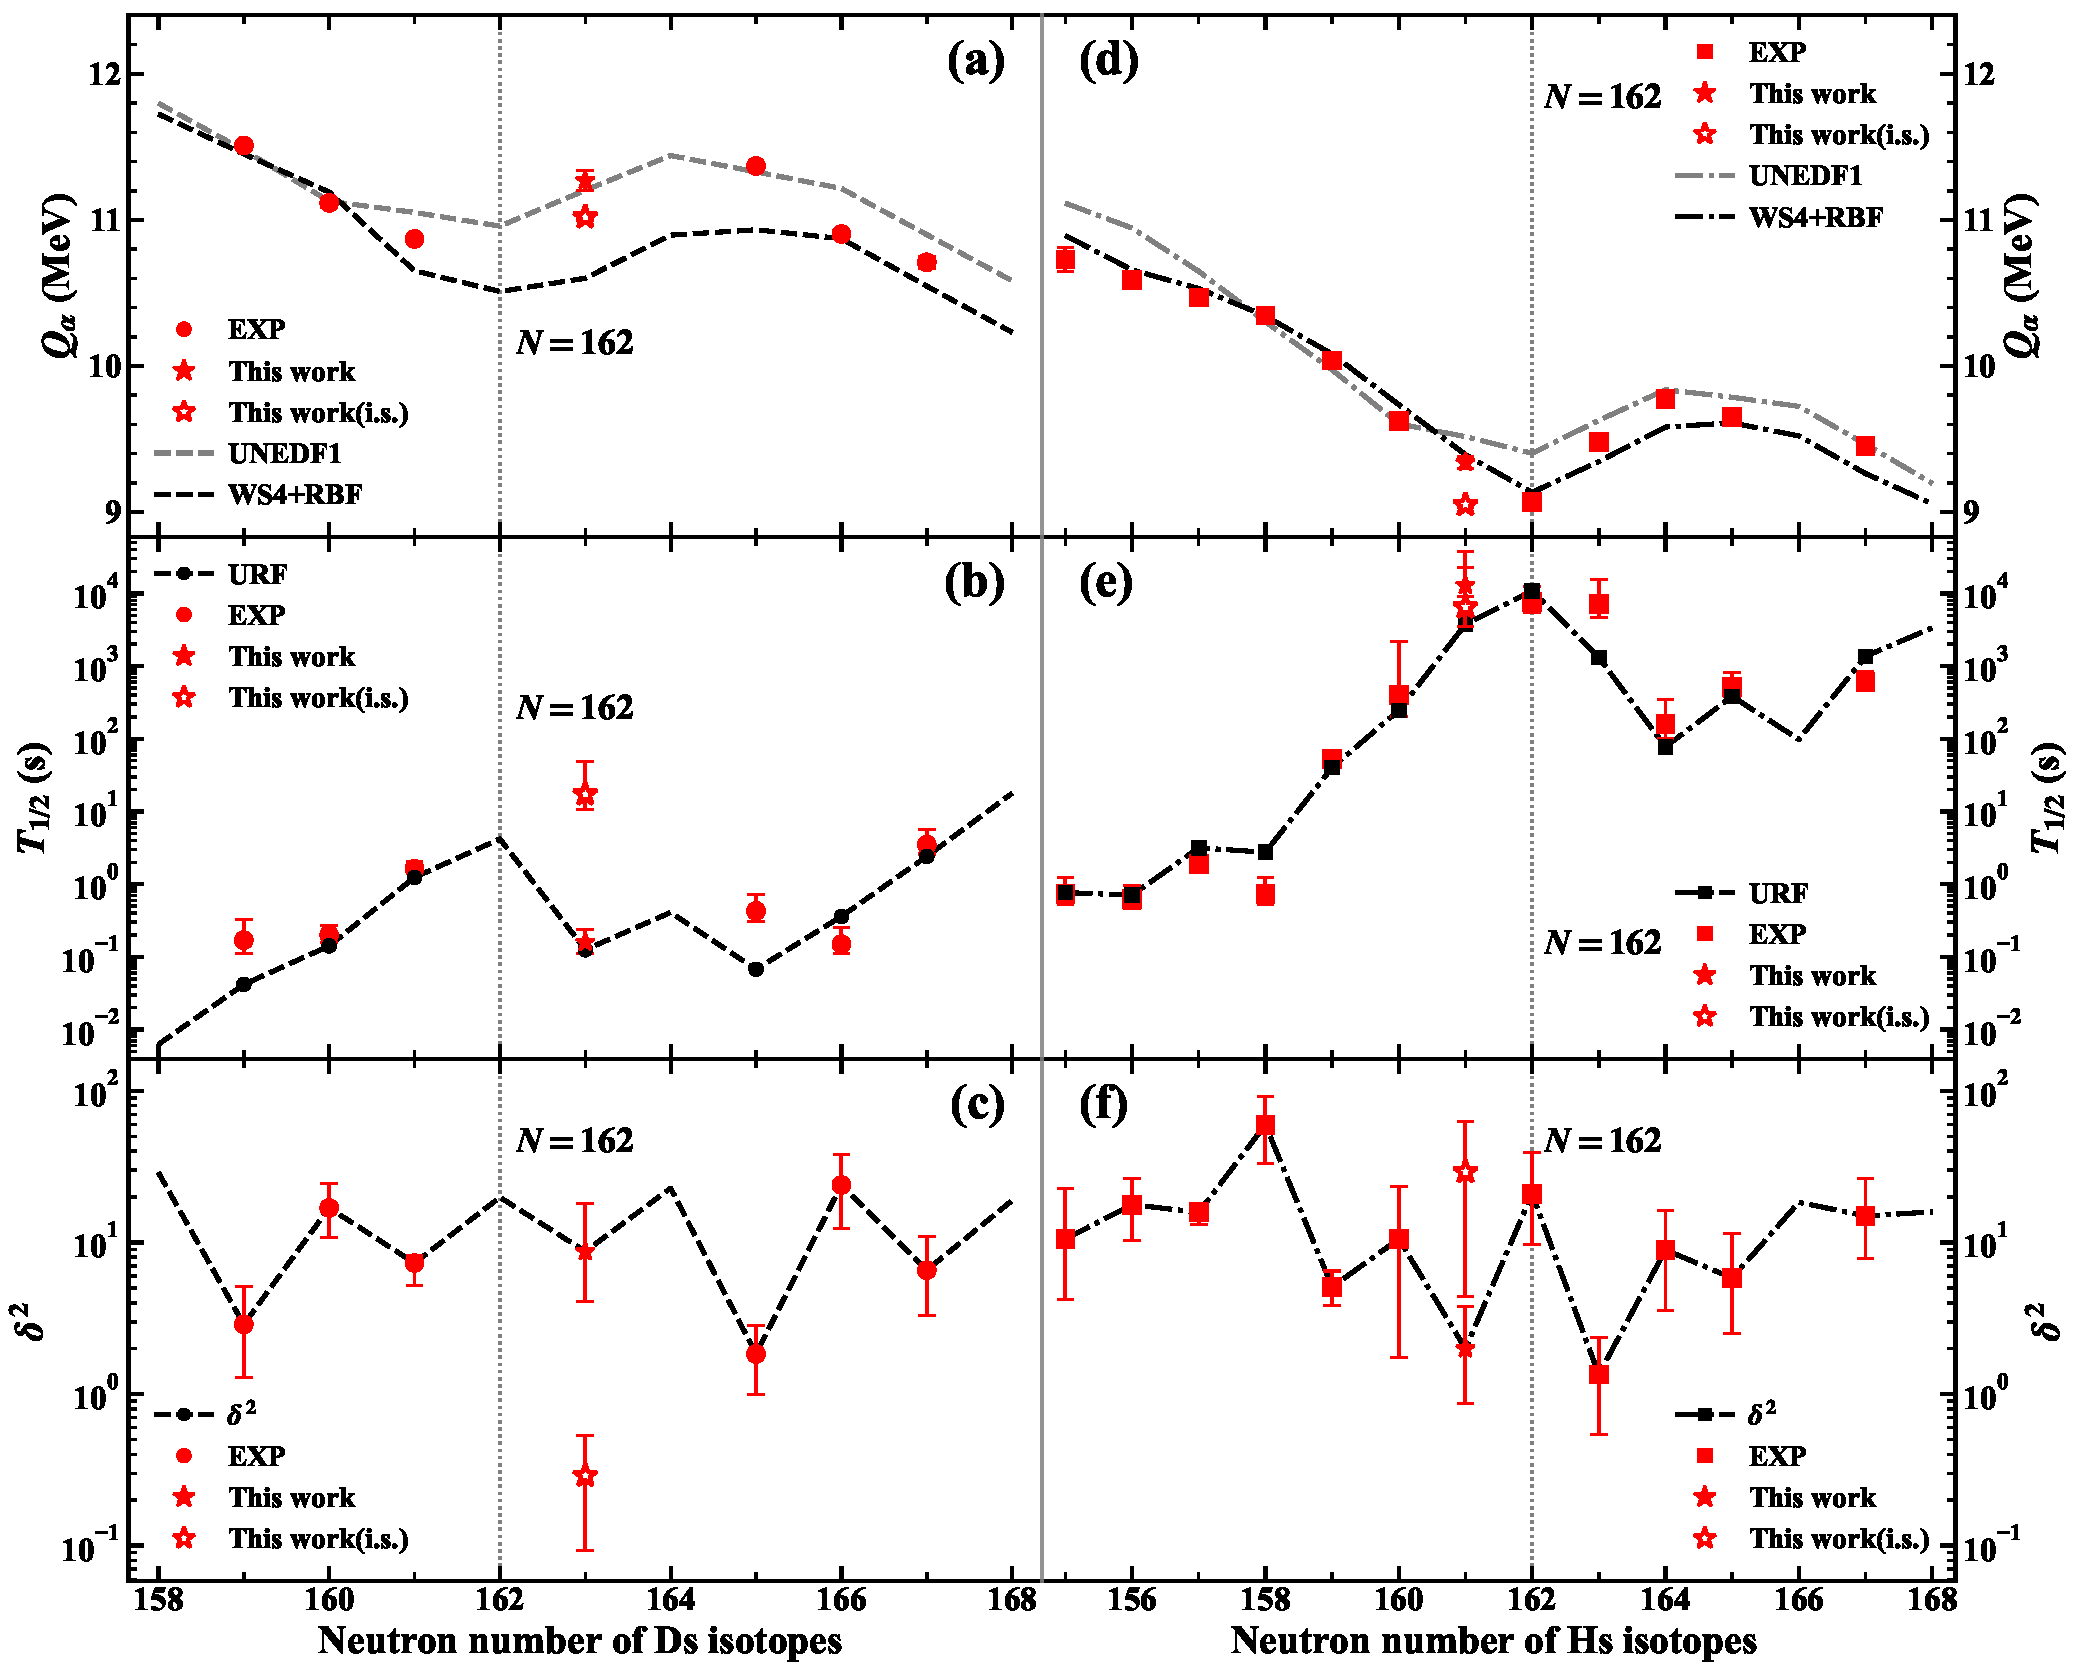
\includegraphics[width=1\textwidth]{System.pdf}
\caption{Systematics of $Q_{\alpha}$, $T_{1/2}$, and reduced $\alpha$-decay width $\delta^{2}$ for the Ds and Hs isotopic chains. 
Panels (a)--(c) correspond to Ds isotopes, and panels (d)--(f) correspond to Hs isotopes. The upper, middle, and lower rows show $Q_{\alpha}$, $T_{1/2}$, and $\delta^{2}$, 
respectively, as functions of neutron number. Experimental values are compared with the UNEDF1 \cite{UNEDF1} and WS4+RBF \cite{WS4+RBF} calculations in the $Q_{\alpha}$ panels 
and with universal Royer formula(URF) values \cite{Deng2020} in the half-life panels. 
The plotted $\delta^{2}$ values are reduced $\alpha$-decay widths evaluated with the Rasmussen method \cite{rasmussen1959AlphaDecayBarrierPenetrabilities}, 
in which the barrier penetrability is calculated in the WKB approximation. Filled stars denote the branches assigned in the present work, and open stars denote the tentative isomeric branches. 
The vertical dotted lines indicate $N = 162$.Data are taken from Refs.~\cite{ackermann2026DecaySpectroscopyHeavy}}
\label{fig:System}
\end{figure*}


The most direct experimental result of the present work is the observation of two distinct decay patterns in $^{273}\mathrm{Ds}$. One branch has a higher $\alpha$-decay energy and a shorter lifetime, whereas the other has a lower $\alpha$-decay energy and a longer lifetime. When the present chains are considered together with the chains reported in Ref.~\cite{oganessian2024SynthesisDecayProperties}, this separation is difficult to reconcile with a single-state interpretation. The decay pattern of $^{269}\mathrm{Hs}$ is also nonuniform. The high and low-energy groups are populated with different relative intensities in direct production and in the decay of $^{273}\mathrm{Ds}$, and no clear cross feeding is observed between $^{273}\mathrm{Ds}^{a}$ and $^{269}\mathrm{Hs}^{a+b}$ or between $^{273}\mathrm{Ds}^{b}$ and $^{269}\mathrm{Hs}^{c}$. Such selectivity is consistent with configuration-dependent $\alpha$ decay. The higher-energy, shorter-lived branch of $^{273}\mathrm{Ds}$ is assigned to
\begin{align*}
^{273}\text{Ds}^{b} &\xrightarrow{\alpha} {}^{269}\text{Hs}^{a,b} \xrightarrow{\alpha} {}^{265}\text{Sg}^{b} \xrightarrow{\alpha} {}^{261}\text{Rf}^{b} \xrightarrow{\text{SF}} \text{fission},
\end{align*}
whereas the lower-energy, longer-lived branch is assigned to
\begin{align*}
^{273}\text{Ds}^{a} &\xrightarrow{\alpha} {}^{269}\text{Hs}^{c} \xrightarrow{\alpha} {}^{265}\text{Sg}^{b} \xrightarrow{\alpha} {}^{261}\text{Rf}^{b} \xrightarrow{\text{SF}} \text{fission}.
\end{align*}

A plausible interpretation is that the long-lived branch of $^{273}\mathrm{Ds}$ has an intrinsic structure different from that of the short-lived branch. In a strongly deformed odd-$N$ nucleus, the $\alpha$-decay rate is governed not only by $Q_{\alpha}$, but also by angular-momentum change, the overlap between the initial and final intrinsic configurations, and hindrance in $\alpha$ formation and barrier penetration \cite{clark2023RoleQuasiparticleStructure}. Therefore, a marked lifetime difference between two branches of the same nuclide can occur even when the difference in $Q_{\alpha}$ is modest. In this context, the observed separation between $^{273}\mathrm{Ds}^{a}$ and $^{273}\mathrm{Ds}^{b}$ is consistent with two competing neutron quasiparticle configurations, one of which gives rise to a hindered, longer-lived $\alpha$ decay.

This interpretation is especially relevant to the shell structure around the deformed $N = 162$ gap \cite{guoStabilizationDeformedSuperheavy2024}. The nucleus $^{273}\mathrm{Ds}$ contains one neutron particle above this gap, whereas $^{269}\mathrm{Hs}$ corresponds to one neutron hole below it. The decay chain $^{273}\mathrm{Ds} \rightarrow {}^{269}\mathrm{Hs}$ therefore probes the single-particle structure on both sides of the same deformed shell closure. Theoretical calculations indicate that several low-lying high-$\Omega$ neutron configurations may be relevant in this region. In particular, the orbitals $\nu 13/2^{-}[716]$ and $\nu 11/2^{-}[725]$ have been predicted to lie close to the Fermi surface, while macroscopic--microscopic calculations for neighboring odd-$N$ transfermium nuclei also place $\nu 11/2^{-}[725]$ among the low-lying candidates \cite{Shi2014,Parkhomenko2005}. It is therefore reasonable to consider whether the long-lived branch of $^{273}\mathrm{Ds}$ is associated with a high-$\Omega$ one-neutron configuration. This possibility is qualitatively consistent with high-$K$ isomerism in the neighboring deformed superheavy region, as discussed for the $^{270}\mathrm{Ds} \rightarrow {}^{266}\mathrm{Hs}$ decay sequence \cite{xuEnhancedStabilitySuperheavy2004}. At present, however, the data do not allow a unique spin-parity or Nilsson-orbital assignment. Interpretations based on either $\nu 13/2^{-}[716]$ or $\nu 11/2^{-}[725]$, as well as other possibilities, remain open.

Within this interpretation, the decay selectivity observed in $^{269}\mathrm{Hs}$ can be understood naturally. If $^{273}\mathrm{Ds}^{a}$ and $^{273}\mathrm{Ds}^{b}$ correspond to different intrinsic configurations, favored $\alpha$ decay is expected to populate daughter states with similar structures. The proposed $^{269}\mathrm{Hs}^{c}$ state, which appears in the low-energy branch and is preferentially associated with $^{273}\mathrm{Ds}^{a}$, may therefore reflect a corresponding low-lying configuration in the daughter nucleus. In contrast, the higher-energy groups $^{269}\mathrm{Hs}^{a}$ and $^{269}\mathrm{Hs}^{b}$ may be associated mainly with the decay of $^{273}\mathrm{Ds}^{b}$. 
The present data may therefore indicate not only a possible isomeric structure in $^{273}\mathrm{Ds}$, but also a correlated multistate structure in $^{269}\mathrm{Hs}$.
It should be emphasized that the evidence for three distinct states in $^{269}\mathrm{Hs}$ remains tentative, and unresolved subgroups or fine-structure decays to different $^{265}\mathrm{Sg}$ energy levels mixed in the data cannot be excluded.

Additional support comes from the isotopic systematics shown in Fig.~\ref{fig:System}. In a single-configuration picture, $Q_{\alpha}$, $T_{1/2}$, and reduced $\alpha$-decay width are expected to evolve with neutron number along the Ds and Hs isotopic chains. The long-lived branch of $^{273}\mathrm{Ds}$ and the low-energy branch of $^{269}\mathrm{Hs}$ deviate from these local trends, supporting an interpretation in terms of different underlying configurations. The reduced widths are used here only as comparative, model-dependent indicators.% within the Rasmussen method \cite{rasmussen1959AlphaDecayBarrierPenetrabilities}.

\begin{figure}
\centering
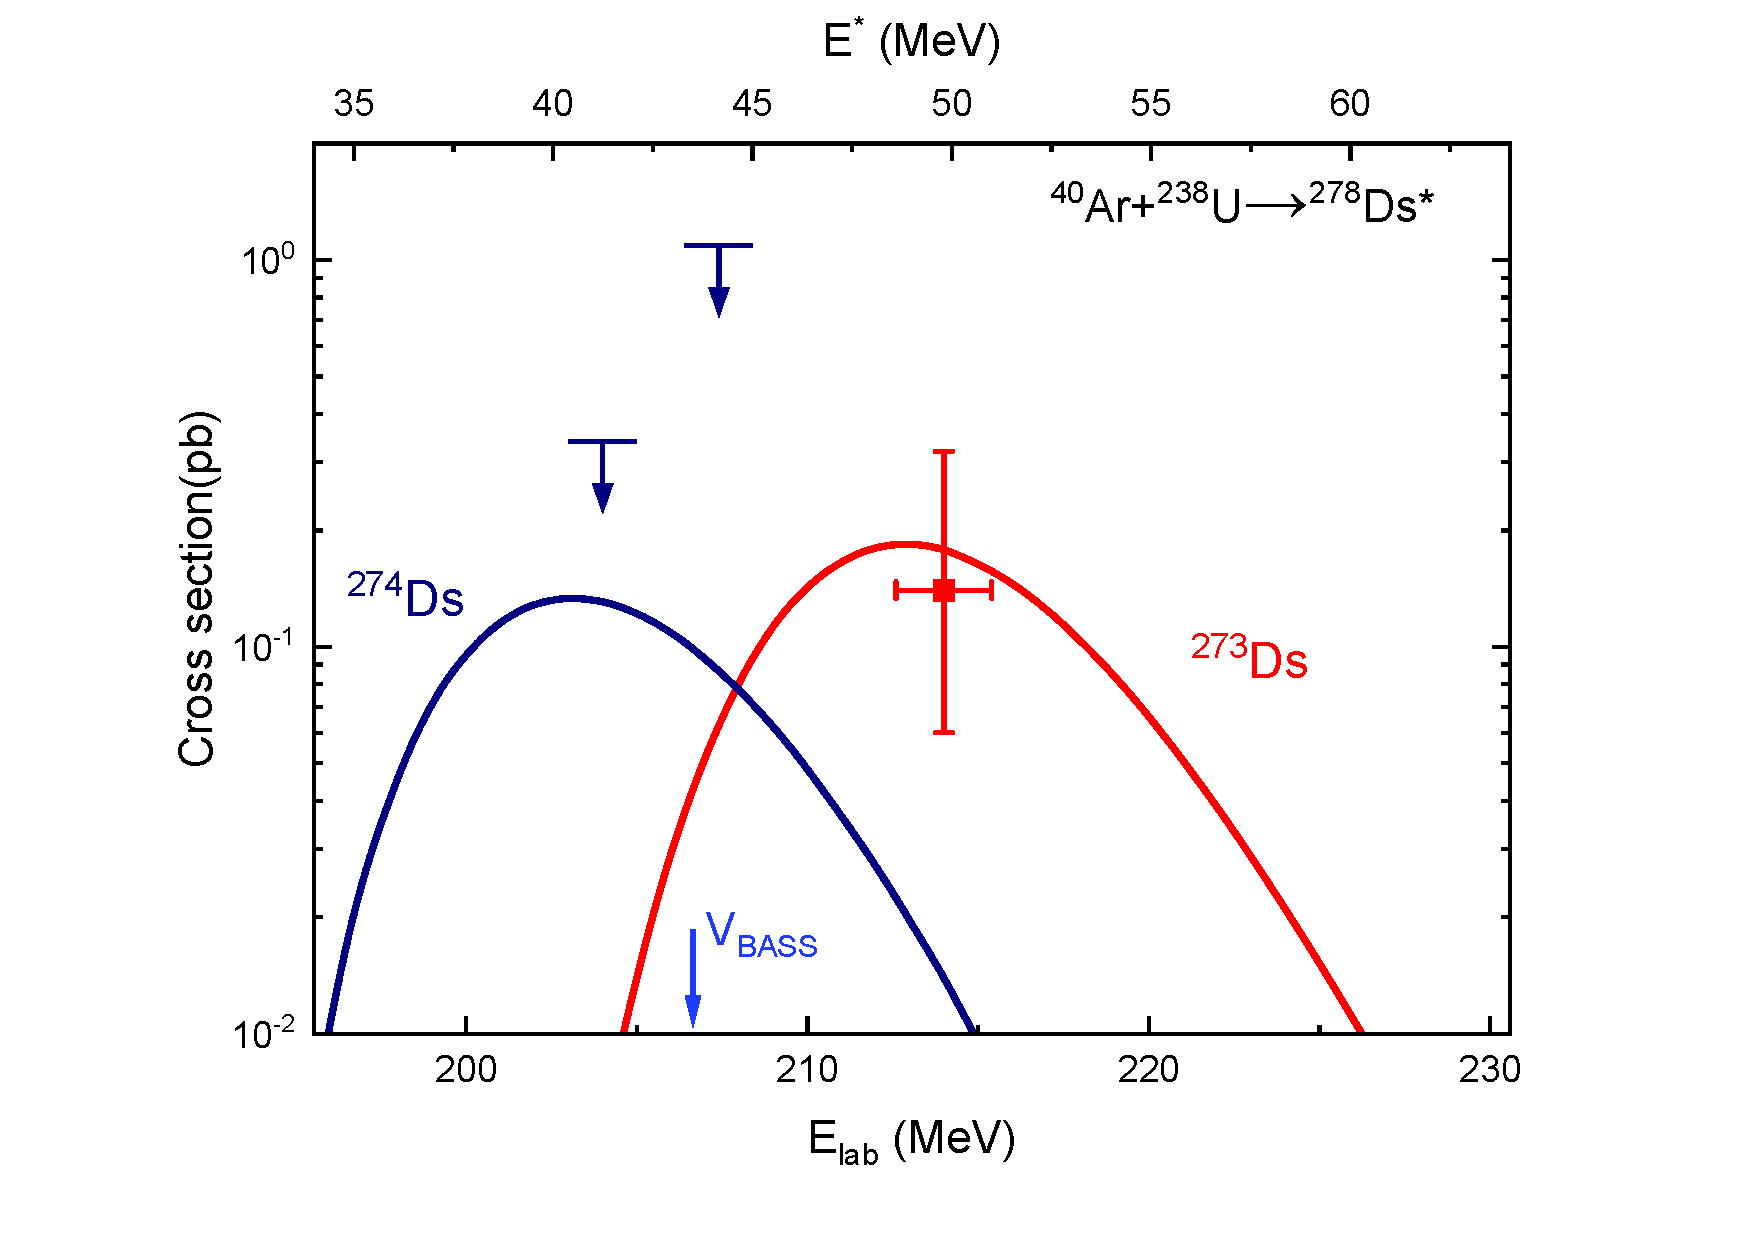
\includegraphics[width=0.5\textwidth]{exFun.pdf}
\caption{Measured cross section and upper limits for the $^{40}$Ar + $^{238}$U $\rightarrow$ $^{278}$Ds$^{*}$ reaction. 
The curves show the calculated excitation functions for the $4n$ and $5n$ channels leading to $^{274}$Ds and $^{273}$Ds with HIVAP calculations\cite{reisdorf1981AnalysisFissionabilityData},
 respectively. The lower horizontal axis gives the laboratory beam energy, and the upper axis gives the corresponding average excitation energy of the compound nucleus. 
 The arrow marked $V_{\mathrm{BASS}}$ indicates the Coulomb barrier estimated with the BASS prescription.}
\label{fig:exFun}
\end{figure}

The excitation-function information provides a further consistency check. As shown in Fig.~\ref{fig:exFun}, the experimental cross sections are broadly consistent with the calculation indicating that the $5n$ channel dominates near the present beam-energy setting. This agreement supports the assignment of the observed chains to $^{273}\mathrm{Ds}$ produced in the $^{238}$U($^{40}$Ar, $5n$)$^{273}$Ds reaction, rather than to neighboring evaporation channels. Although the excitation function alone cannot distinguish different intrinsic states, it shows that the long- and short-lived branches are populated within the same reaction framework. This favors a structural origin for the difference between the two branches. The absence of an observed $^{274}\mathrm{Ds}$ chain is also not unexpected. With a transmission efficiency of 20\%, an $\alpha$-detection efficiency of 87(6)\%, and the present beam dose, the current upper limits do not yet strongly constrain the calculated $4n$ excitation function. A weak $^{274}\mathrm{Ds}$ yield would also be consistent with the sub-barrier character of the $4n$ channel, for which fusion proceeds through quantum tunneling.

In summary, the present data support a picture in which $^{273}\mathrm{Ds}$ has two distinct decay branches and $^{269}\mathrm{Hs}$ may contain at least one additional low-energy state beyond the previously recognized high-energy groups. A consistent interpretation is that odd-$N$ nuclei around the deformed $N = 162$ shell closure exhibit configuration-dependent $\alpha$ decay, possibly involving high-$\Omega$ structures related to the $\nu 13/2^{-}[716]$ and $\nu 11/2^{-}[725]$ orbitals. If confirmed by future high-statistics measurements and dedicated structure calculations, this interpretation would extend the evidence for low-lying isomeric structures in the transfermium region and provide new constraints on the single-particle level ordering near the deformed $N = 162$ shell gap.

\section{Summary and conclusions}

A beam-energy scan of the $^{238}$U($^{40}$Ar, $4n$--$5n$)$^{274,273}$Ds reaction was performed at SHANS-2. No correlated decay chain attributable to $^{274}\mathrm{Ds}$ was identified at excitation energies of 42 and 45 MeV, and upper limits of 0.34 and 1.1 pb were obtained. At 50 MeV, two complete decay chains of $^{273}\mathrm{Ds}$ were observed, and the extracted $5n$-channel cross section of $0.14^{+0.18}_{-0.08}$ pb agrees with the value reported previously for the same reaction at DGFRS-2 \cite{oganessian2024SynthesisDecayProperties}.

One observed chain follows the higher-energy, shorter-lived branch of $^{273}\mathrm{Ds}$, whereas the other corresponds to a lower-energy, longer-lived branch. When the present data are combined with previous results, the evidence supports two distinct decay branches in $^{273}\mathrm{Ds}$, with the lower-energy branch interpreted as a candidate low-lying isomeric state.

The daughter nucleus $^{269}\mathrm{Hs}$ shows a parent-dependent population pattern. In addition to the previously recognized high-energy groups, the present work identifies a low-energy event at 8.915(22) MeV that is preferentially connected with the longer-lived branch of $^{273}\mathrm{Ds}$. Although the statistics remain limited, this behavior is compatible with an additional low-lying state in $^{269}\mathrm{Hs}$.

The isotopic systematics of $Q_{\alpha}$, $T_{1/2}$, and reduced $\alpha$-decay width in the Ds and Hs chains further support a structural change near $N = 162$. The overall picture is consistent with configuration-dependent $\alpha$ decay in odd-$N$ transfermium nuclei and provides constraints on the ordering of low-lying neutron quasiparticle orbitals around the deformed $N = 162$ shell gap. More definitive conclusions will require higher-statistics direct-production measurements and dedicated structure calculations.

\begin{acknowledgments}
The authors would like to thank the accelerator crew of CAFE2 for providing the stable $^{40}$Ar beam.
\end{acknowledgments}

\bibliography{example}

\end{document}
